% !TeX root = ../main.tex
\section{Introduction}
\label{sec:intro}
Sequential Recommendation (SR), which drives next-item suggestions on Web platforms such as e-commerce and streaming services, models evolving user preferences through sequence-level Collaborative Filtering (CF), learning transition patterns that capture which items follow a given interaction history.
Traditional ID-based models~\cite{sasrec,gru4rec,fmlp} learn these transitions from interactions alone, which makes them vulnerable to data sparsity and cold-start items.
Meanwhile, items on these platforms come with rich content, including titles and images.
This content across consecutive items reveals \textit{preference continuity}, such as a recurring color or style, and thus explains why transitions occur.

Content-based SR exploits these contents to capture preference continuity and to alleviate the data sparsity and cold-start problems of ID-based models.
% Early multimodal SR models feed item features from small pretrained encoders such as BERT~\cite{bert} and CLIP~\cite{clip} into an SR backbone~\cite{mmrec1,modrec_m3srec,modrec_hm4sr}, but these encoders view each item in isolation and offer limited semantic understanding.
To do so, multimodal SR models~\cite{mmrec1,modrec_m3srec,modrec_hm4sr} feed item features from small pretrained encoders such as BERT~\cite{bert} and CLIP~\cite{clip} into an SR backbone such as SASRec~\cite{sasrec}, yet these encoders view each item in isolation and offer limited semantic understanding.
Recently, Large Language Models (LLMs) read the titles in a history with strong text understanding, capturing textual continuity and substantially improving SR~\cite{slim,llm2rec}.
However, LLMs read only text and thus cannot exploit visual continuity in item images.
Feeding CLIP image features into an LLM~\cite{illmrec} does not fully resolve this limitation, because the LLM interprets these features within its text space and compresses each image into a single token, discarding fine-grained details.

Unlike these LLM-based approaches, Large Vision--Language Models (VLMs)~\cite{qwen2.5-vl,internvl3} directly process raw images and text, which makes them well suited to multimodal SR for three reasons.
\textbf{First}, large-scale vision--language pretraining provides rich visual semantics and cross-modal priors.
\textbf{Second}, VLMs' strong multi-image reasoning lets them jointly compare the images in a user's sequence and capture visual continuity, such as a recurring color or style.
\textbf{Third}, they accept images together with textual instructions, so a prompt such as ``Describe this item image sequence'' can guide them to understand an image history for recommendation.
For these reasons, we apply VLMs to SR so that they read users' multimodal histories and exploit both textual and visual continuity.

However, applying VLMs directly to recommendation leaves a problem inherent to them: \textbf{modality collapse}.
% Recent studies use VLMs to rank candidate items directly~\cite{mllmmsr,hanorec} or to derive item representations~\cite{notellm2,vlm_prompt}, but VLMs are known to over-rely on the dominant modality, usually text, while underusing the weaker one~\cite{modality_bias1,modality_gap_gen1,modality_gap_emb3}.
They are known to over-rely on the dominant modality, usually text, while underusing the weaker one~\cite{modality_bias1,modality_gap_gen1}, even as recent studies use them to rank candidate items directly~\cite{mllmmsr,hanorec} or to derive item representations~\cite{notellm2,vlm_prompt}.
Our experiments (Sec.~\ref{sec:empirical}) show that this collapse in vanilla VLMs hampers recommendation: visual embeddings barely separate the next item from negatives, and adding image embeddings to the text embeddings can even lower accuracy (i.e., a negative transfer).
% Thus, the collapse weakens the influence of the visual modality and undermines the very multimodality that motivates VLMs, leaving visual continuity overlooked for recommendation; resolving it is essential.
Thus, the collapse undermines the very multimodality that motivates VLMs, leaving visual continuity overlooked for recommendation; resolving it is crucial.

% Yet standard contrastive supervised fine-tuning (SFT)~\cite{infonce1}, an essential step for adapting VLMs to SR, further amplifies this collapse, as our analysis of accuracy, gradients, and embedding geometry shows (Sec.~\ref{sec:empirical}).
Yet we find that standard contrastive Supervised Fine-Tuning (SFT)~\cite{infonce1}, an essential step for adapting VLMs to SR, further amplifies this collapse (Sec.~\ref{sec:empirical}).
SFT updates increasingly follow the text gradient, widening the gradient gap between text and vision, which suggests that the VLM takes the easier text modality as a \textit{shortcut}~\cite{shortcut2} to reduce the loss.
As a result, the visual modality loses even more of its ability to separate each user's next item from negatives, and text-only inputs outperform vision-only inputs by a widening margin.
The negative transfer thus becomes consistent: adding image embeddings to the text embeddings lowers accuracy on both datasets (Fig.~\ref{fig:drop_grad} left).
To fully exploit the cross-modal capabilities of VLMs for recommendation, we need an objective that, unlike standard SFT, corrects this collapse.

% To this end, we propose \textbf{VLM2Rec} (Sec.~\ref{sec:methods}), which corrects the collapse by strengthening each user's weaker modality and aligning each user's relative similarity structure over the same items in the two modality spaces.
To this end, we propose \textbf{VLM2Rec} (Sec.~\ref{sec:methods}), which corrects the collapse with two objectives.
\textit{Weak-modality Penalized Contrastive Learning} ($\mathcal{L}_{\text{WPCL}}$) identifies the weaker modality of each user, since users differ in how much they rely on textual or visual cues, and strengthens it with a penalty weight that grows with its gap from the stronger modality.
\textit{Cross-modal Relational Topology Regularization} ($\mathcal{L}_{\text{CRTR}}$) softly aligns the neighborhood of each user's history in the two modality spaces without forcing identical text and vision embeddings, so that fusing them improves recommendation.
Moreover, we introduce $\text{VLM2Rec}_{\text{plug}}$, which transfers the trained item embeddings to SR backbones and thus serves without VLM calls at the latency of conventional SR models (Sec.~\ref{sec:deployment}).
Experiments (Sec.~\ref{sec:exp}) show that VLM2Rec mitigates the collapse across benchmarks and consistently improves accuracy and robustness.
The main contributions of this paper are as follows:
\begin{itemize}[leftmargin=*]
    \item We empirically find that standard contrastive SFT, though essential for adapting VLMs to SR, amplifies their modality collapse by under-optimizing the weaker modality.
    \item We propose VLM2Rec, which strengthens each user's weaker modality and aligns each user's relative similarity structure in the two modality spaces; its variant $\text{VLM2Rec}_{\text{plug}}$ enhances SR backbones with the item embeddings while matching the serving latency of conventional SR models.
    \item We demonstrate the effectiveness of VLM2Rec through extensive experiments across datasets, SR backbones, and VLM families.
\end{itemize}

% Figure: drop_grad analysis (modality dropout test + gradient dynamics).
\begin{figure*}[t]
    \centering
    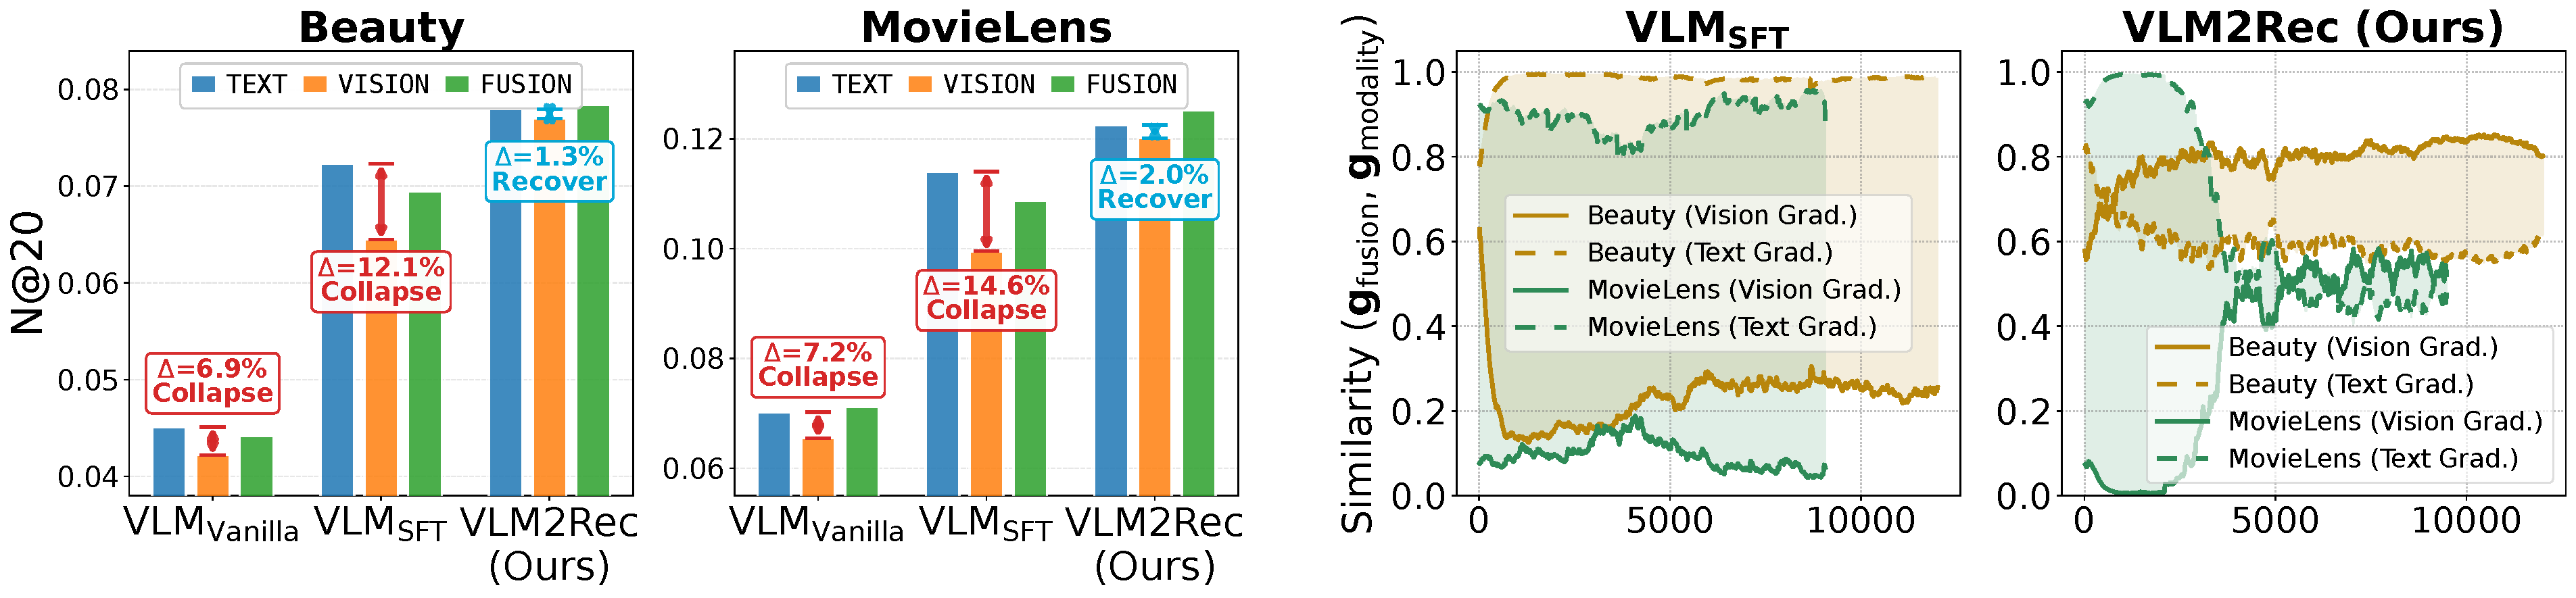
\includegraphics[width=\textwidth]{figures/drop_grad.pdf}
    \Description{Bar charts compare recommendation performance with text-only, vision-only, and fused inputs on Beauty and MovieLens. Line charts compare the alignment of text and vision gradients with the fused gradient during SFT and VLM2Rec training.}
    \caption{Analysis of modality collapse in the VLM2Rec setting (N@20): dropout test (Left) and gradient dynamics (Right). $\text{VLM}_{\text{SFT}}$ widens the \TEXTset{}--\VISIONset{} gap and favors text gradients; VLM2Rec (ours) narrows it and rebalances updates.}
    \label{fig:drop_grad}
\end{figure*}